\documentclass[a4paper,12pt]{article}
\usepackage{graphicx}
\usepackage[a4paper,margin=1in]{geometry}
\usepackage{titlesec}
\usepackage{hyperref}
\usepackage{amsmath}    % For math environments and symbols
\usepackage{amssymb}    % For \mathbb and other math symbols
\usepackage{amsfonts}   % Additional math fonts
\usepackage[backend=biber,style=numeric,sorting=none]{biblatex}

\addbibresource{references.bib} % Add references.bib with the appropriate entries

% Title format
\titleformat{\section}{\large\bfseries}{\thesection}{1em}{}

% Title settings
\title{
    \includegraphics[scale=0.4]{Cam_logo_bw.png}\\
    \vspace{0.5cm}
    C1 Research Computing - Coursework Assignment
}
\author{Raunaq Rai (rsr45@cam.ac.uk)\\
    Data Intensive Science, Department of Physics, University of Cambridge
}
\date{18 December, 2024}

\begin{document}

\maketitle

\section{Introduction}
This report details the development and implementation of a Python package, \texttt{dual\_autodiff}, designed for automatic differentiation using dual numbers. The package computes derivatives efficiently while supporting mathematical operations such as trigonometric, logarithmic, and exponential functions.

The approach builds on the concept of forward-mode automatic differentiation, which is essential in fields like optimisation, computational physics, and machine learning. This technique traces its roots to the foundational work by Wengert~\cite{wengert1964automatic}, who introduced a systematic way to compute derivatives using intermediate variables. More recently, Baydin et al.~\cite{baydin2018automatic} surveyed the use of automatic differentiation in machine learning, emphasising its importance in training deep neural networks.

To enhance performance, a Cython-optimised version, \texttt{dual\_autodiff\_x}, was also developed. This document covers the structure of the project, the mathematical principles behind dual numbers, and the implementation details of the package.

\section{Setting Up the Development Environment}

Apple Silicon devices primarily use the ARM64 architecture, which can pose challenges when working with scientific computing tools built for x86\_64. To ensure compatibility with these tools, I configured the development environment to run in x86\_64 mode. This step enabled the execution of packages and tools designed for x86\_64 systems.

To achieve this:
\begin{itemize}
    \item \textbf{Rosetta Installation:} Rosetta, an emulation layer, was installed to facilitate running x86\_64 binaries on ARM-based devices. This was achieved using:
    \begin{verbatim}
    /usr/sbin/softwareupdate --install-rosetta
    \end{verbatim}
    \item \textbf{Configuring Terminal:} The Terminal application was set to run in Rosetta mode, ensuring compatibility with x86\_64 libraries and tools.
    \item \textbf{Creating an x86\_64 Conda Environment:} A dedicated Conda environment was created with all required dependencies for developing and testing the package.
\end{itemize}

This setup allowed for consistent development and ensured the compatibility of tools and libraries required for this project. Further details can be found within dual\_autodiff.html within docs.

\section{Theoretical Background}

\subsection{Dual Numbers}
Dual numbers can be defined as truncated Taylor series of the form:
\begin{equation}
    x = v + \dot{v}\epsilon,
    \label{eq:dual_number_form}
    \end{equation}
where \(v, \dot{v} \in \mathbb{R}\), and \(\epsilon\) is a nilpotent number such that \(\epsilon^2 = 0\) and \(\epsilon \neq 0\). Here:
\begin{itemize}
    \item \(v\): Represents the \textit{primal value}.
    \item \(\dot{v}\): Represents the \textit{derivative} or \textit{tangent value}.
\end{itemize}

As explained by Baydin et al.~\cite{baydin2018automatic}, arithmetic operations with dual numbers align naturally with symbolic differentiation principles:
\begin{equation}
    (x_1 + \dot{x}_1\epsilon) + (x_2 + \dot{x}_2\epsilon) = (x_1 + x_2) + (\dot{x}_1 + \dot{x}_2)\epsilon,
    \label{eq:dual_addition}
    \end{equation}
    
    \begin{equation}
    (x_1 + \dot{x}_1\epsilon)(x_2 + \dot{x}_2\epsilon) = x_1x_2 + (x_1\dot{x}_2 + \dot{x}_1x_2)\epsilon,
    \label{eq:dual_multiplication}
    \end{equation}
    

\subsection{Automatic Differentiation}
Automatic differentiation uses dual numbers to compute derivatives efficiently. For a function \(f(x)\), substituting \(x = v + \dot{v}\epsilon\) yields:
\begin{equation}
    f(x) = f(v + \dot{v}\epsilon) = f(v) + f'(v)\dot{v}\epsilon,
    \label{eq:dual_function}
    \end{equation}
    
The derivative \(f'(v)\) is embedded in the coefficient of \(\epsilon\), enabling evaluation of function values and derivatives.

This principle extends to composite functions via the chain rule:
\begin{equation}
    f(g(v + \dot{v}\epsilon)) = f(g(v)) + f'(g(v))g'(v)\dot{v}\epsilon,
    \label{eq:composite_function}
    \end{equation}
    

    \section{Implementation of Dual Numbers and Operations}

    \subsection{Overview of the \texttt{Dual} Class}
    The \texttt{dual.py} file implements the \texttt{Dual} class, the core of the \texttt{dual\_autodiff} package. This class defines dual numbers and supports operations such as addition, subtraction, multiplication, and division.
    
    \subsubsection{Arithmetic Operations}
    The \texttt{Dual} class simplifies arithmetic operations by overriding standard operators such as \texttt{+}, \texttt{-}, \texttt{*}, and \texttt{/}. This allows \texttt{Dual} objects to be used just like regular numbers. For example:
    \begin{verbatim}
    x = Dual(2, 1)
    y = Dual(3, 2)
    print(x + y)  # Output: Dual(real=5, dual=3)
    \end{verbatim}
    
    \subsubsection{Mathematical Functions}
    The \texttt{Dual} class also implements important mathematical functions such as:
    \begin{itemize}
        \item Trigonometric functions (\texttt{sin}, \texttt{cos}, \texttt{tan}).
        \item Exponential and logarithmic functions (\texttt{exp}, \texttt{log}).
        \item Hyperbolic functions (\texttt{sinh}, \texttt{cosh}, \texttt{tanh}).
        \item Square root (\texttt{sqrt}).
    \end{itemize}
    For example:
    \begin{verbatim}
    x = Dual(2, 1)
    result = x.sin()
    print(result)  # Output: Dual(real=0.9092..., dual=-0.4161...)
    \end{verbatim}
    
    \subsubsection{Error Handling and Special Cases}
    The \texttt{Dual} class ensures that mathematical operations like \texttt{log} and \texttt{sqrt} are only applied within valid domains, raising appropriate errors when encountering invalid inputs.
    
    \subsection{Example of Using Dual Numbers}
    Consider the function:
    \begin{equation}
        f(x) = \log(x) + x^2 \implies f'(x) = \frac{1}{x} + 2x.
        \label{eq:derivative_example}
    \end{equation}
    
    This can be evaluated directly using the \texttt{Dual} class:
    \begin{verbatim}
    x = Dual(2, 1)
    f_x = x.log() + x**2
    print(f_x)  # Output: Dual(real=4.0, dual=4.5)
    \end{verbatim}
    
    \subsection{Utility Functions}
    
    To enhance usability and simplify mathematical operations, two utility modules are provided as part of the package:
    
    \begin{itemize}
        \item \texttt{functions.py}: This module provides aliases for commonly used mathematical functions, such as \texttt{sin}, \texttt{cos}, \texttt{log}, and \texttt{sqrt}. These aliases act as wrappers around the corresponding methods of the \texttt{Dual} class, allowing users to apply these functions directly to \texttt{Dual} instances or standard numerical values. For example:
        \begin{verbatim}
        from dual_autodiff.functions import sin, cos, log
        x = Dual(2, 1)
        result = sin(x) + log(x)
        \end{verbatim}
        These aliases improve the user experience by making the library's API intuitive and easy to use, especially when working with dual numbers in complex expressions.
    
        \item \texttt{base.py}: This module includes helper functions to streamline operations on \texttt{Dual} instances:
        \begin{itemize}
            \item \texttt{is\_dual\_instance(value)}: A utility function that checks whether a given value is an instance of the \texttt{Dual} class. This is useful for validation, ensuring that mathematical operations are applied only to compatible types.
            \item \texttt{ensure\_dual(value)}: A function that wraps a non-\texttt{Dual} value into a \texttt{Dual} object with its derivative initialised to zero. This ensures that all mathematical functions can seamlessly handle both standard numerical values and dual numbers.
        \end{itemize}
    \end{itemize}
    
    These utility functions simplify the use of the package by enabling both explicit handling of dual numbers and implicit conversions when required, making the library more accessible for a wide range of users.
    

\section{Project Structure and Packaging}

\subsection{Repository Organisation}
The repository adheres to established best practices for Python projects to ensure clarity, maintainability, and modularity. Below is an overview of its structure:

\subsubsection{Top-Level Directory}
The top-level directory organises the project as follows:
\begin{itemize}
    \item \textbf{\texttt{dual\_autodiff/}}: Core implementation, including modules like \texttt{dual.py}, \texttt{functions.py}, and \texttt{base.py}.
    \item \textbf{\texttt{dual\_autodiff\_x/}}: Cythonised implementation of the package for enhanced performance, including \texttt{.pyx} source files and compiled \texttt{.so} binaries.
    \item \textbf{\texttt{tests/}}: Unit tests for core modules. Use the \texttt{pytest} command to run the tests.
    \item \textbf{\texttt{docs/}}: Documentation files, including Sphinx configurations and example notebook.
    \item \textbf{\texttt{report/}}: LaTeX report and related files.
    \item \textbf{\texttt{dist/}}: Package distribution files (wheel and source archives).
    \item \textbf{\texttt{build/}}: Temporary build files.
    \item \textbf{\texttt{pyproject.toml}}: Modern Python project configuration.
    \item \textbf{\texttt{requirements.txt}}: Python dependencies.
    \item \textbf{\texttt{environment.yaml}}: Conda environment definition.
    \item \textbf{\texttt{README.md}}: Project overview and instructions.
    \item \textbf{\texttt{LICENCE}}: Contains the MIT License under which the project is distributed.
\end{itemize}



\subsection{Building and Installing the Package}
The \texttt{pyproject.toml} file is used to manage the configuration and metadata of the project. It follows the modern Python packaging standards and includes the following sections:
\begin{itemize}
    \item \texttt{[build-system]}: Specifies the tools required for building the package, such as \texttt{setuptools} and \texttt{wheel}.
    \item \texttt{[project]}: Contains metadata, including the project name, version, author, and dependencies.
    \item \texttt{[tool.setuptools\_scm]}: Enables dynamic versioning based on the state of the repository.
\end{itemize}

To build and install the package, the following steps were performed:
\begin{enumerate}
    \item Install build tools: \texttt{pip install build}.
    \item Build distributions: \texttt{python -m build}.
    \item Install in editable mode: \texttt{pip install -e .}.
\end{enumerate}

This approach ensures the package is properly configured, packaged, and ready for distribution or further development.

\section{Publishing to PyPI}

To make the \texttt{dual\_autodiff} package publicly available, it was uploaded to the Python Package Index (PyPI). The following steps outline the publishing process and installation instructions.

\subsection{Publishing to PyPI}

To publish the \texttt{dual\_autodiff} package on PyPI, the following steps were followed:

\begin{enumerate}
    \item \textbf{Create Distributions:}
    Build source and wheel distributions as done previously:

    \item \textbf{Upload to PyPI:}
    Use \texttt{twine} to securely upload distributions.
    
    Authentication with PyPI credentials was required.

    \item \textbf{Verify Upload:}
    \url{https://pypi.org/project/rsr45-dual-autodiff/}
\end{enumerate}

\subsection{Installing the Package}
Install the package via \texttt{pip}:
\begin{verbatim}
pip install rsr45-dual-autodiff
\end{verbatim}

\subsection{Testing the Installation}
Verify functionality:
\begin{verbatim}
import dual_autodiff as df
x = df.Dual(2, 1)
print(x.sin())
\end{verbatim}



\section{Differentiating a Function}

\subsection{Function Definition}
The target function for differentiation is:
\begin{equation}
    f(x) = \log(\sin(x)) + x^2 \cos(x),
    \label{eq:function_definition}
    \end{equation}
    
The derivative of this function, computed analytically, is:
\begin{equation}
    f'(x) = \frac{\cos(x)}{\sin(x)} -x^2 \sin(x) + 2x \cos(x),
    \label{eq:function_derivative}
    \end{equation}
    

\subsection{Using Dual Numbers for Differentiation}
To compute \(f'(x)\) at \(x = 1.5\) using dual numbers:
\begin{itemize}
    \item Represent \(x\) as a dual number: \(x = 1.5 + 1\epsilon\), where the real part is \(1.5\) and the dual part represents the derivative.
    \item Substitute \(x\) into \(f(x)\) and use the dual number arithmetic to compute \(f'(x)\) from the dual part of the result.
\end{itemize}

\subsection{Results}

\subsubsection{Using Dual Numbers}
The function \(f(x)\) and its derivative \(f'(x)\) were computed at \(x = 1.5\) using dual numbers. The results are as follows:
\[
f(1.5) = 0.15665054756073515, \quad f'(1.5) = -1.9612372705533612
\]

\subsubsection{Using Manual Computation}
The analytical expression for \(f(x)\) and \(f'(x)\) was used to compute the same values at \(x = 1.5\). The results are:
\[
f(1.5) = 0.15665054756073515, \quad f'(1.5) = -1.9612372705533614
\]

\subsubsection{Comparison}
The results obtained using dual numbers closely match the manually computed values, confirming the correctness of the dual number implementation. The slight discrepancy in the derivative (\(2 \times 10^{-13}\)) is attributed to floating-point precision errors inherent in numerical computations.

\subsection{Comparison with Numerical Differentiation}

\begin{itemize}
    \item \textbf{Numerical Differentiation:} The central difference formula was used:
    \begin{equation}
        f'(x) \approx \frac{f(x + h) - f(x - h)}{2h},
        \label{eq:central_difference}
    \end{equation}
    
    This was evaluated for step sizes decreasing logarithmically from \(h = 10^{-0.5}\) to \(h = 10^{-3}\).
\end{itemize}

Figure~\ref{fig:convergence_derivative} illustrates the behavior of the numerical derivative as the step size decreases. The red dashed line represents the true derivative obtained using dual numbers, which serves as the reference value.

\begin{figure}[h!]
    \centering
    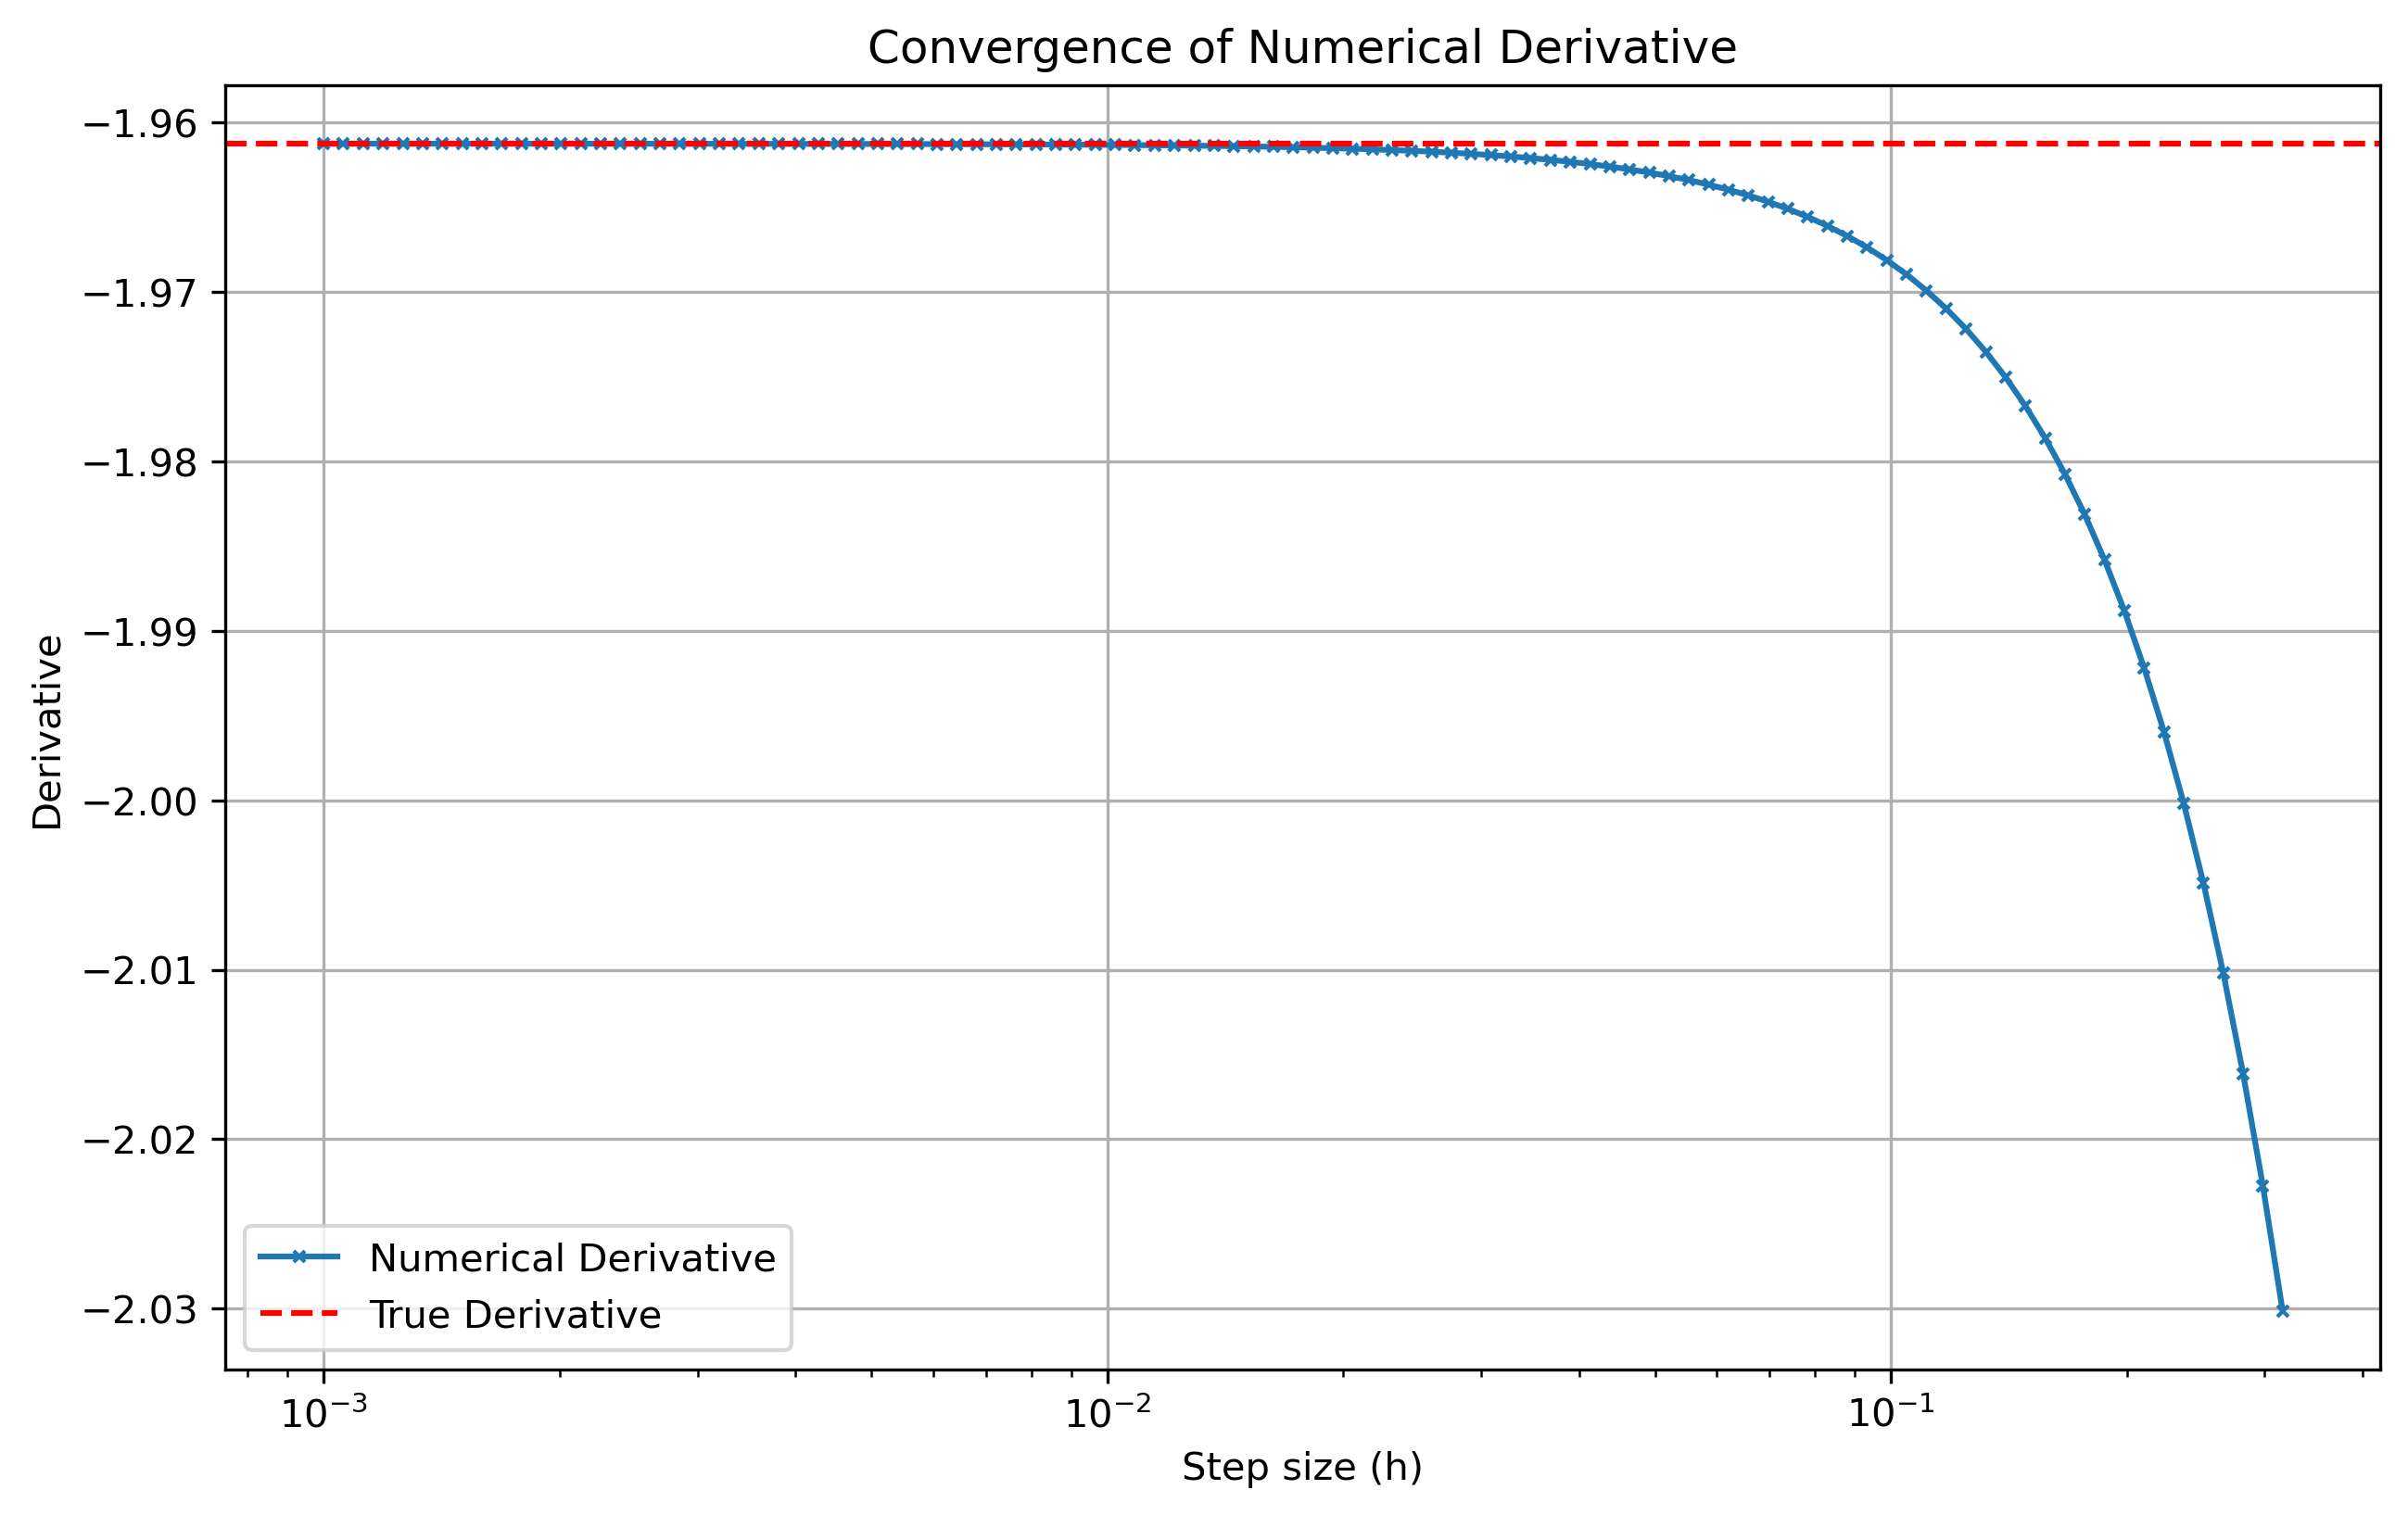
\includegraphics[width=0.8\textwidth]{convergence_derivative.png}
    \caption{Divergence of the numerical derivative for increasing step sizes. The red dashed line indicates the true derivative obtained using dual numbers. The numerical derivative converges to the true value for small step sizes (approximately \(< 10^{-2}\)), but diverges due to round-off errors as \(h\) becomes larger.}
    \label{fig:convergence_derivative}
\end{figure}

\begin{itemize}
    \item \textbf{Accuracy:} For moderate values of \(h\), the numerical derivative closely matches the true value. However, as \(h\) increases further, round-off errors lead to divergence.
    \item \textbf{Dual Numbers:} The dual number method provides a stable and precise derivative, unaffected by the limitations of finite differences.
    \item \textbf{Efficiency:} Unlike numerical differentiation, dual numbers compute the derivative in a single step, making the method both computationally efficient and less error-prone.
\end{itemize}

\section{Tests and Validation}

The \texttt{tests/} directory contains unit tests designed to validate the functionality of the \texttt{dual\_autodiff} package. These tests ensure the correctness of mathematical operations, dual number functionality, and integration with various functions like trigonometric, logarithmic, and exponential operations.

\subsection{Structure of the \texttt{tests/} Directory}
The directory includes the following key test files:
\begin{itemize}
    \item \texttt{test\_dual.py}: Validates the core \texttt{Dual} class, including arithmetic operations and function implementations.
    \item \texttt{test\_functions.py}: Tests global mathematical functions like \texttt{sin}, \texttt{cos}, and \texttt{log}.
    \item \texttt{test\_base.py}: Ensures utility functions such as \texttt{is\_dual\_instance()} and \texttt{ensure\_dual()} work correctly.
\end{itemize}

\subsection{Outcome}
The tests validate that the \texttt{dual\_autodiff} package functions as expected under various scenarios. They also confirm that dual numbers provide accurate derivatives.

\section{Project Documentation with Sphinx}

The \texttt{docs/} directory contains all the files required to generate the HTML documentation for the \texttt{dual\_autodiff} package using Sphinx. After running \texttt{make html} in the terminal, Sphinx processes the source files and generates structured HTML documentation, which can be found in the \texttt{build/html/} directory.

\subsection{Structure of the \texttt{docs/} Directory}
\begin{itemize}
    \item \texttt{Makefile} and \texttt{make.bat}: Used to build the documentation. The \texttt{Makefile} is for Unix-based systems, while \texttt{make.bat} is for Windows.
    \item \texttt{source/}: Contains the source files for the documentation:
    \begin{itemize}
        \item \texttt{index.rst}: The main landing page of the documentation, linking to other sections.
        \item \texttt{dual\_autodiff.rst}: API reference for the package, generated using the \texttt{autodoc} extension.
        \item \texttt{modules.rst}: Lists all the modules included in the \texttt{dual\_autodiff} package.
        \item \texttt{tutorial.rst}: A guide for using the package, linking to the tutorial notebook.
        \item \texttt{dual\_autodiff.ipynb}: A Jupyter notebook providing hands-on examples of the package's features. This also includes a comparison with the package's cythonized version.
        \item \texttt{implementation.rst}: Documentation of the theoretical background and implementation details of the package.
        \item \texttt{apple\_silicon\_x86\_setup.rst}: A section explaining how to set up the development environment on Apple Silicon devices.
        \item \texttt{conf.py}: The Sphinx configuration file, which defines project settings, extensions, and theme configurations.
    \end{itemize}

    \item \texttt{build/}: Stores the generated documentation:
    \begin{itemize}
        \item \texttt{build/doctrees/}: Contains intermediate files generated during the build process.
        \item \texttt{build/html/}: The final HTML output, including:
\begin{itemize}
    \item \texttt{index.html}: Main landing page.
    \item \texttt{dual\_autodiff.html}: API reference.
    \item \texttt{tutorial.html}: Examples and usage guide.
    \item \texttt{apple\_silicon\_x86\_setup.html}: Environment setup instructions.
    \item \texttt{implementation.html}: Theoretical background and implementation.
    \item \texttt{modules.html}: Package modules overview.
    \item \texttt{\_images/}: Documentation figures (\texttt{dual\_autodiff\_13\_1.png}, \texttt{dual\_autodiff\_23\_1.png}).
    \item \texttt{\_modules/}: Generated module docs (\texttt{dual\_autodiff/base.html}, \texttt{dual\_autodiff/dual.html}, etc.).
    \item \texttt{\_sources/}: Source files (\texttt{index.rst.txt}, \texttt{tutorial.rst.txt}, etc.).
    \item \texttt{\_static/}: Static assets (CSS, JavaScript).
    \item \texttt{search.html}, \texttt{genindex.html}, \texttt{searchindex.js}: Search and index functionality.
\end{itemize}

    \end{itemize}
\end{itemize}

\subsection{Generated Output}
The generated HTML documentation includes:
\begin{itemize}
    \item \textbf{Main Landing Page:} Provides an overview of the project with links to tutorials, references, and key sections.
    \item \textbf{API Documentation:} Comprehensive details for all modules, classes, and functions in the package.
    \item \textbf{User Tutorial:} A practical guide with examples demonstrating how to use the package effectively.
    \item \textbf{Setup Guide:} Step-by-step instructions for configuring the development environment, including Apple Silicon devices.
    \item \textbf{Implementation Details:} An in-depth explanation of the internal workings, including key algorithms and design principles.
\end{itemize}


The Sphinx-generated documentation ensures clarity and accessibility. It combines automatically generated API references with user-friendly tutorials, making it an important resource for both developers and users.

\section{Cythonizing the Package}

\subsection{Configuration and Implementation}
To Cythonize the \texttt{dual\_autodiff} package, a separate directory named \texttt{dual\_autodiff\_x} was created. This included necessary configurations to ensure efficient compilation and distribution of the Cythonized version.

\subsubsection{Key Configuration Files}
\begin{itemize}
    \item \textbf{\texttt{setup.py}:} Defined Cython modules to be compiled (e.g., \texttt{dual.pyx}, \texttt{functions.pyx}) and metadata for the package.
    \item \textbf{\texttt{pyproject.toml}:} Declared build dependencies (\texttt{Cython}, \texttt{setuptools}, \texttt{wheel}) and Python version compatibility.
    \item \textbf{\texttt{MANIFEST.in}:} Included essential files (\texttt{README.md}, compiled \texttt{.so} files) while excluding unnecessary source files (\texttt{.pyx}, \texttt{.py}).
\end{itemize}

\subsubsection{Cythonization Process}
\begin{enumerate}
    \item \textbf{Code Preparation:} 
    Python files (\texttt{.py}) in the original \texttt{dual\_autodiff} directory were copied into \texttt{dual\_autodiff\_x} and renamed to \texttt{.pyx} to allow Cython compilation.
    
    \item \textbf{Compilation:} 
    The source files were compiled into shared object files (\texttt{.so}) using:
    \begin{verbatim}
    python setup.py build_ext --inplace
    \end{verbatim}
    
    \item \textbf{Installation:} 
    The package was installed in editable mode for testing and further development:
    \begin{verbatim}
    pip install -e .
    \end{verbatim}
\end{enumerate}

\subsection{Performance Insights}
To evaluate the effectiveness of Cythonization, we compared the performance of the pure Python and Cythonized implementations.

\subsubsection{Experimental Setup}
Execution times were measured for arrays of dual numbers with lengths ranging from 100 to 14,000. Three ranges of real parts were considered: \((0,10)\), \((10,100)\), and \((100,1000)\). Each experiment was repeated 100 times, and linear regression was applied to analyse gradients of execution time with respect to array length.

\subsubsection{Observations}
Figure~\ref{fig:performance_comparison} illustrates the performance comparison:
\begin{itemize}
    \item The Cythonized version exhibited lower execution times across all scenarios.
    \item Gradients for the Cythonized implementation were consistently smaller, highlighting better scalability.
    \item Performance improvements were particularly notable for larger arrays, validating the computational efficiency of Cython.
\end{itemize}

\begin{figure}[h!]
    \centering
    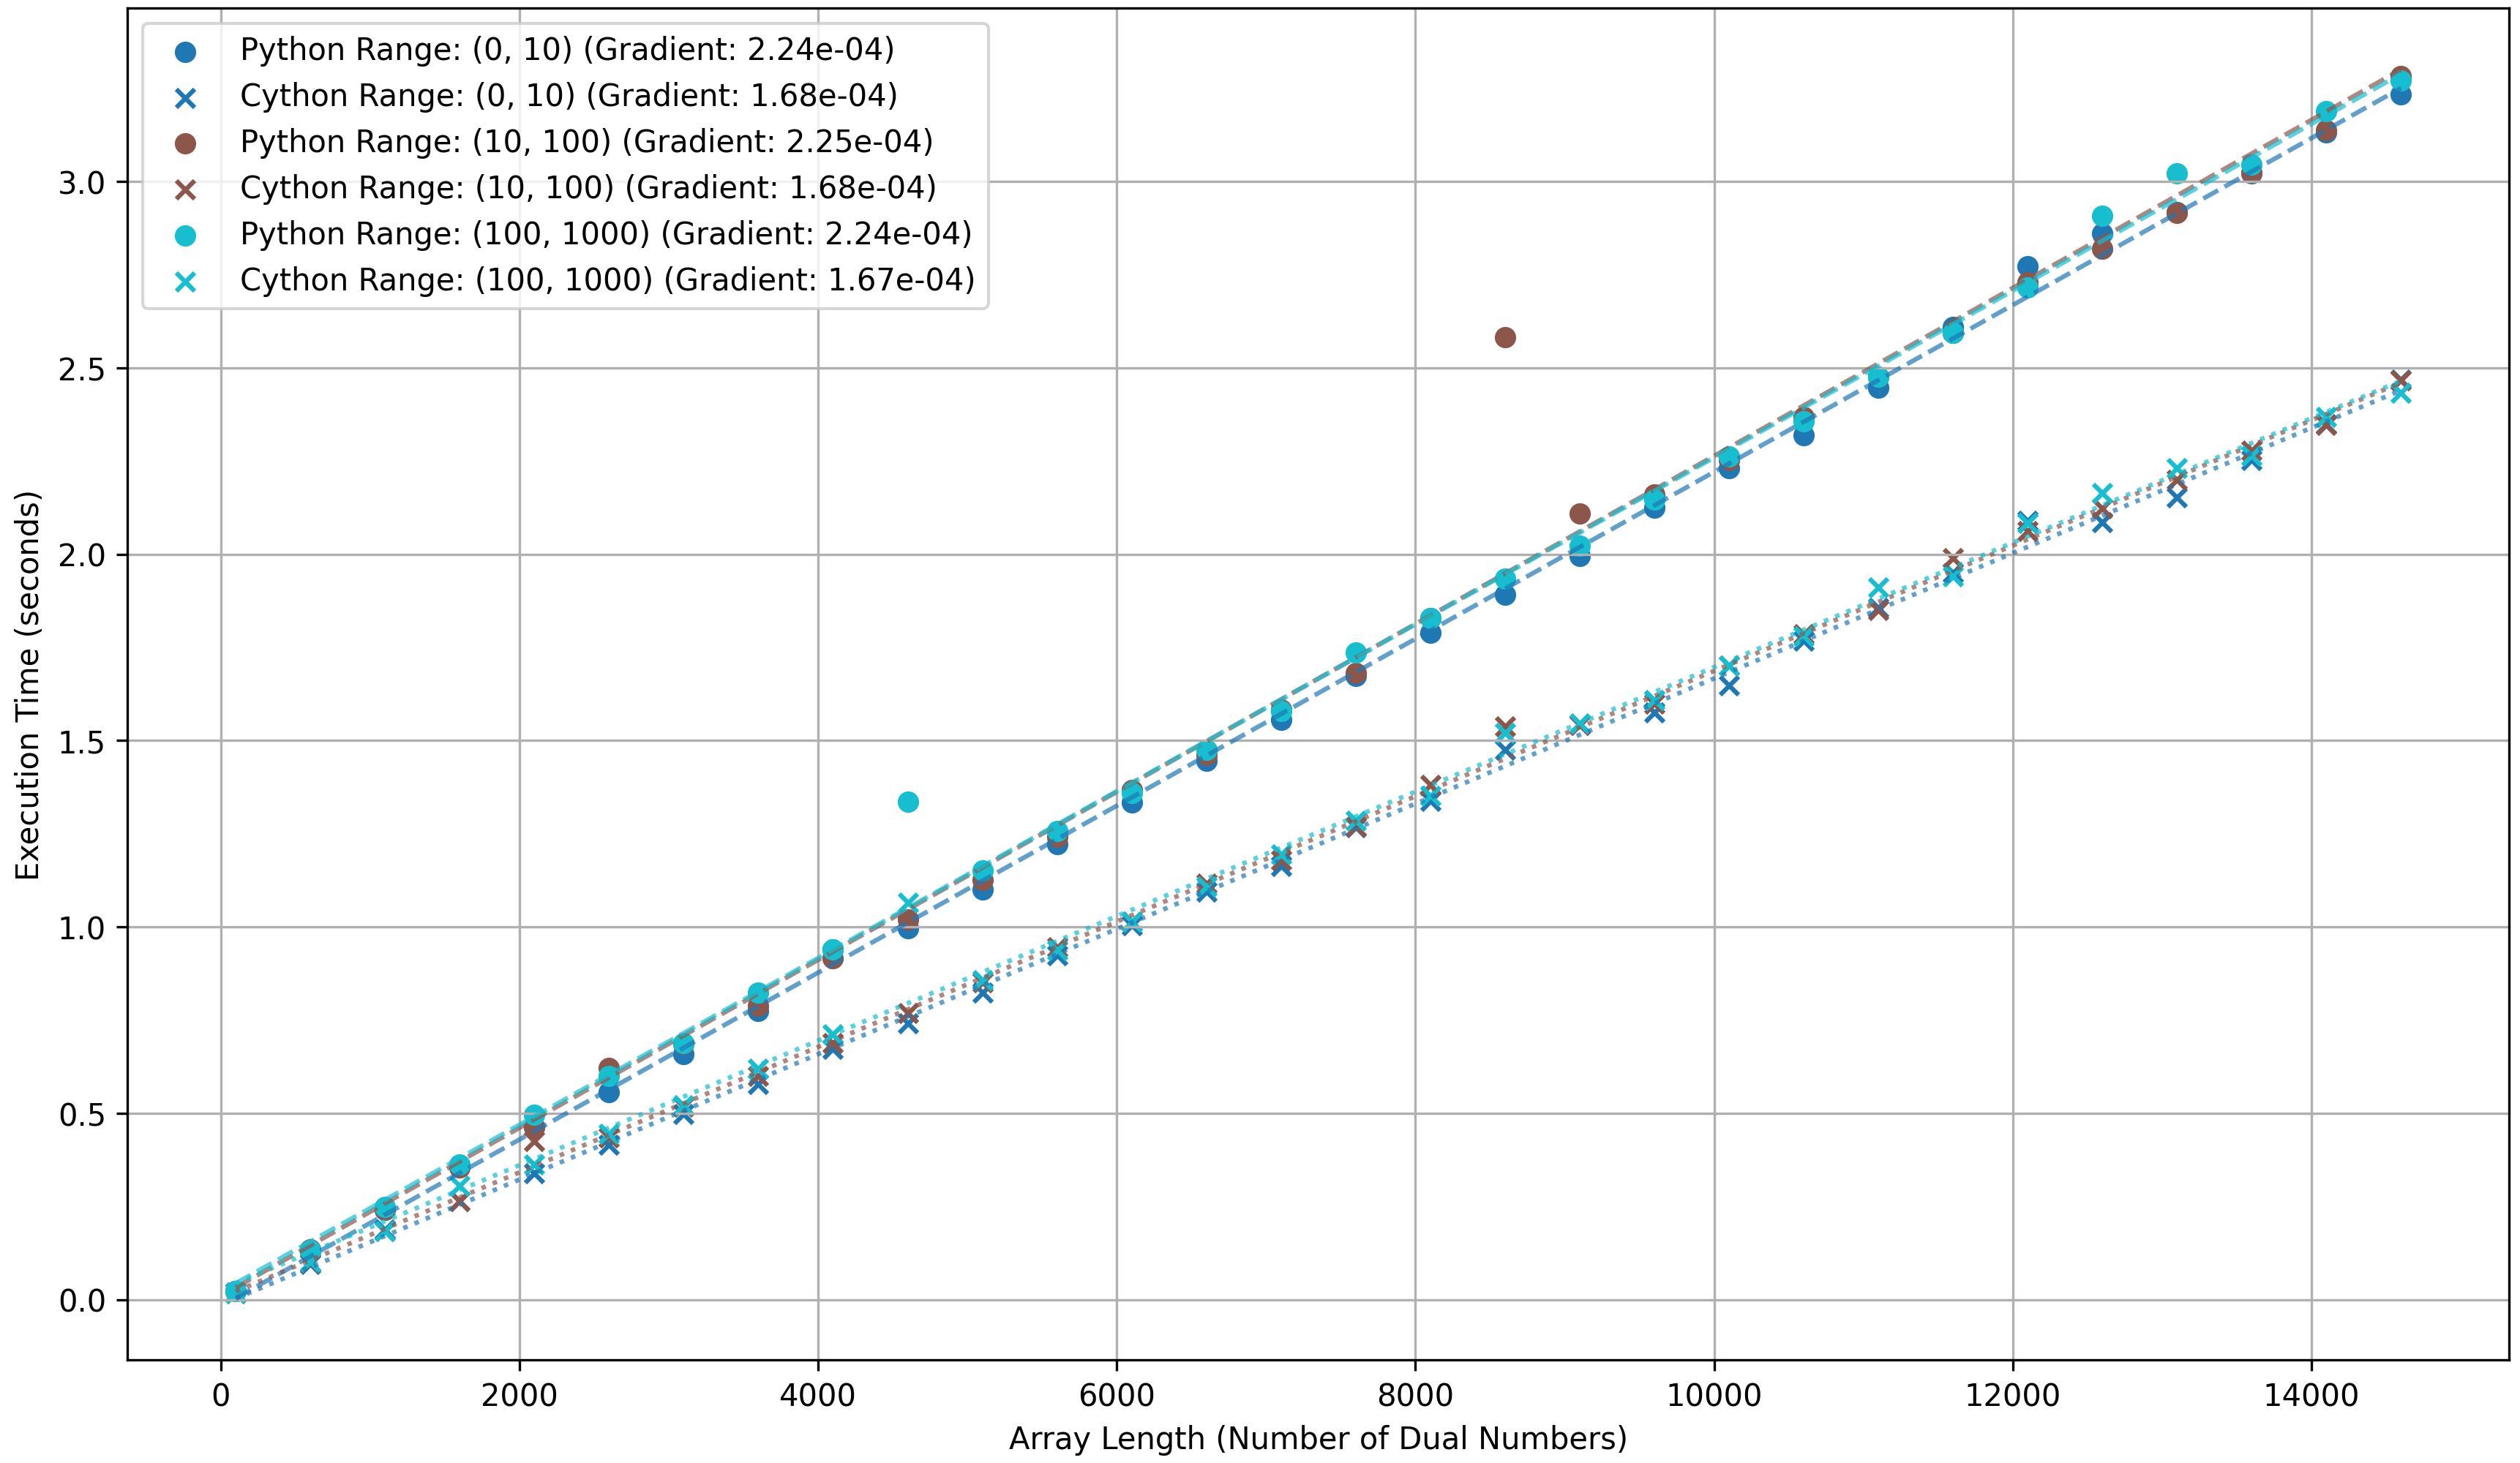
\includegraphics[width=0.8\textwidth]{performance_comparison.png}
    \caption{Performance comparison between the pure Python and Cythonized versions of \texttt{dual\_autodiff}. The gradients indicate the rate of increase in execution time with array length.}
    \label{fig:performance_comparison}
\end{figure}

\subsection{Analysis of Gradients}
The gradients in Figure~\ref{fig:performance_comparison} provide a quantitative measure of how execution time scales with the array length:

\begin{itemize}
    \item \textbf{Python Implementation:} The gradients are consistently higher, around \(2.20 \times 10^{-4}\), across all ranges of dual numbers. This indicates that the execution time for the Python implementation increases more rapidly with the number of dual numbers. The similarity of gradients across ranges suggests that the range of real parts has minimal impact, and the computational overhead primarily depends on array length.
    
    \item \textbf{Cythonized Implementation:} The gradients are significantly lower, approximately \(1.63 \times 10^{-4}\), for all ranges. This slower rate of increase in execution time highlights the efficiency of the Cythonized implementation. A lower gradient indicates that the Cythonized version scales better with increasing array lengths, making it more suitable for handling larger datasets.
\end{itemize}

\textbf{Scalability and Impact of Lower Gradients:} \\
The lower gradient for the Cythonized implementation demonstrates its superior scalability. As the array length grows, the execution time for the Cythonized version increases at a much slower rate compared to the Python implementation. This efficiency arises from the reduced overhead in Cython, where the code is compiled into C, minimising dynamic type-checking and interpretation, which are inherent to Python. Consequently, the Cythonized version is better equipped to handle larger and more computationally intensive tasks efficiently.

\subsection{Conclusion}
Cythonization significantly reduced execution time and enhanced scalability by converting Python code into optimized C extensions. These improvements align with findings from prior research, such as Mortensen and Langtangen~\cite{mortensen2016cython}, which highlight that Cythonized code can achieve performance levels comparable to low-level languages like C++. While additional experiments could provide further insights, Figure~\ref{fig:performance_comparison} clearly illustrates that the Cythonized implementation consistently outperforms the Python version, with the performance gap widening as array lengths increase.


\section{Building Wheels for Linux}

To create specific wheels for the \texttt{dual\_autodiff\_x} package targeting \texttt{cp310-manylinux\_x86\_64} and \texttt{cp311-manylinux\_x86\_64}, I initially attempted the process manually on the University of Cambridge's CSD3 cluster due to compatibility issues on macOS M4. Later, I streamlined the process by utilizing a family member's laptop, which allowed me to generate wheels in the required manylinux format with a single command.

The initial steps on CSD3 taught me valuable lessons about creating environments, understanding computer architecture, and troubleshooting compatibility challenges. Although these steps did not produce manylinux-compatible wheels, the experience deepened my technical understanding and problem-solving skills. Borrowing an older laptop ultimately provided a simpler and more effective solution, highlighting the importance of adaptability in software development.

Below, I outline my approach to building wheels manually on CSD3 without using \texttt{cibuildwheel}. While the resulting wheels, included in my \texttt{wheelhouse} directory, are not in manylinux format, the process was a valuable learning experience. In section~11.2, I outline how I was able to build the wheels more easily and in the correct format.

I have included four \texttt{.whl} files in the \texttt{wheelhouse} directory. However, the two essential files are those in the manylinux format, as they meet the required compatibility standards and are required for the coursework.

\subsection{Steps for Building the Wheels on CSD3}
\begin{enumerate}
    \item \textbf{Building the Python 3.10 Wheel:}
    \begin{itemize}
        \item Python 3.10 was built from source and installed in \texttt{\$HOME/python310}:
        \begin{verbatim}
        ./configure --prefix=$HOME/python310 --enable-optimisations
        make -j$(nproc) && make install
        \end{verbatim}
        \item The wheel was created and saved in the \texttt{wheelhouse} directory:
        \begin{verbatim}
/home/rsr45/python310/bin/python3.10 setup.py bdist_wheel 
--dist-dir wheelhouse
        \end{verbatim}
    \end{itemize}

    \item \textbf{Building the Python 3.11 Wheel:}
    \begin{itemize}
        \item Verified Python 3.11 was installed on CSD3 and prepared the environment:
        \begin{verbatim}
        python3.11 -m pip install --user --upgrade pip setuptools 
        wheel cython
        \end{verbatim}
        \item The wheel was created and saved in the \texttt{wheelhouse} directory:
        \begin{verbatim}
        python3.11 setup.py bdist_wheel --dist-dir wheelhouse
        \end{verbatim}
    \end{itemize}
\end{enumerate}


\subsection{Final Method and Contents of the Wheel}

By utilising a family member's laptop, I generated both wheels in the manylinux format with a single command:
\begin{verbatim}
CIBW_BUILD="cp310-manylinux_x86_64 cp311-manylinux_x86_64" cibuildwheel
 --output-dir wheelhouse
\end{verbatim}
The \texttt{CIBW\_BUILD} environment variable specifies that the wheels should be built exclusively for Python 3.10 and Python 3.11 on the manylinux\_x86\_64 platform. This command uses \texttt{cibuildwheel}, which uses Docker (running in the background) to build compatible wheels efficiently, and outputs the generated wheels to the \texttt{wheelhouse} directory. 

This method simplified the process and ensured compliance with \texttt{manylinux} standards, resulting in wheels suitable for distribution across most Linux environments. The wheels contain only the necessary compiled files (\texttt{.so} and \texttt{.pyd}), with source files (\texttt{.pyx}) excluded, as verified by inspecting the wheel contents.

The wheels are stored in the \texttt{wheelhouse} directory, and their contents were verified by extracting each into the \texttt{wheel\_contents} directory:
\begin{itemize}
    \item \textbf{Compiled Binaries:} Shared object files (\texttt{*.so}) for the core modules (\texttt{base}, \texttt{dual}, \texttt{functions}, and \texttt{version}), compiled for both \texttt{x86\_64-linux-gnu} (manylinux-compatible) and \texttt{darwin} (macOS). These binaries ensure platform compatibility.
    \item \textbf{Metadata:} The \texttt{dist-info} directory contains essential metadata files, including:
    \begin{itemize}
        \item \texttt{METADATA}: Provides details about the package, such as name, version, and dependencies.
        \item \texttt{WHEEL}: Specifies compatibility standards and wheel-specific metadata.
        \item \texttt{RECORD}: Contains file integrity information, including hashes and file paths.
    \end{itemize}
\end{itemize}


\subsection{PyPI Upload}

The \texttt{dual\_autodiff\_x} package was uploaded to PyPI under the name \texttt{rsr45-dual-autodiff-x}, allowing users to install it easily via:
\begin{verbatim}
pip install rsr45-dual-autodiff-x
\end{verbatim}

The package is available at the following link: \href{https://pypi.org/project/rsr45-dual-autodiff-x/}{https://pypi.org/project/rsr45-dual-autodiff-x/}

\subsubsection{Key Features}
\begin{itemize}
    \item Efficient dual number arithmetic.
    \item Comprehensive mathematical functions.
    \item Automatic differentiation.
    \item Performance optimisation with Cython for enhanced speed.
\end{itemize}


This ensures the package is accessible for scientific and computational tasks, promoting usability and reproducibility.

\section{Conclusion}

This project successfully implemented the \texttt{dual\_autodiff} package, providing a method for forward-mode automatic differentiation using dual numbers. Through a structured approach, key objectives such as developing the \texttt{Dual} class, performing differentiation, creating a Cythonized version, and packaging the library for Linux via \texttt{cibuildwheel} were accomplished.

The pure Python implementation of the \texttt{dual\_autodiff} package offered ease of use and flexibility, while the Cythonized version (\texttt{dual\_autodiff\_x}) significantly enhanced performance, as demonstrated in the quantitative comparisons. By leveraging \texttt{cibuildwheel}, Linux-compatible manylinux wheels were created, ensuring broad usability across platforms. The package was also uploaded to PyPI, simplifying installation and distribution.

The project emphasised best practices in software development, including testing with \texttt{pytest}, documentation via Sphinx, and the use of modular project structures. Practical examples and performance insights were integrated into a tutorial notebook, ensuring the package's utility in real-world scenarios.

This coursework reinforced critical skills in computational physics, software optimisation, and development workflows. The experience highlighted the importance of adaptability and problem-solving, particularly when addressing compatibility challenges and optimising performance.

Future work could extend the package's capabilities to support higher-order derivatives or alternate differentiation modes. Additionally, further optimisation and support for additional architectures, such as ARM-based platforms, would expand its applicability.

In conclusion, the \texttt{dual\_autodiff} package is an efficient and versatile tool for automatic differentiation, with potential applications in optimisation, machine learning, and computational physics.

\section*{Declaration of Use of AI Tools}

I declare that all ideas, methods, and approaches used in this project were conceived and developed independently through my own research and understanding. The work presented here is entirely my own.

The following AI tools were used solely for support purposes:
\begin{itemize}
    \item \textbf{ChatGPT:} Used to refine code snippets, assist with LaTeX formatting, and improve the clarity and structure of the written report. All content generated by this tool was critically evaluated and adapted as necessary to ensure accuracy and alignment with my original ideas.
    \item \textbf{GitHub Copilot:} Used to suggest coding snippets and assist the implementation of functions. All suggested code was reviewed, modified, and tested to meet the specific requirements of this project.
\end{itemize}

These tools were used strictly to enhance productivity and ensure clarity. They did not contribute to the conceptualisation of the project, the development of ideas, or the formulation of methods, all of which were my own work.



\printbibliography


\end{document}
